% Created 2025-02-16 Sun 17:31
% Intended LaTeX compiler: pdflatex
\documentclass[11pt]{article}
\usepackage[utf8]{inputenc}
\usepackage[T1]{fontenc}
\usepackage{graphicx}
\usepackage{longtable}
\usepackage{wrapfig}
\usepackage{rotating}
\usepackage[normalem]{ulem}
\usepackage{amsmath}
\usepackage{amssymb}
\usepackage{capt-of}
\usepackage{hyperref}
\date{\today}
\title{}
\hypersetup{
 pdfauthor={},
 pdftitle={},
 pdfkeywords={},
 pdfsubject={},
 pdfcreator={Emacs 29.4 (Org mode 9.7.21)}, 
 pdflang={English}}
\begin{document}

\tableofcontents

\section{malwD}
\label{sec:orgcd99897}
A malware detector application written in golang.
\section{How To}
\label{sec:org98509a1}
\begin{itemize}
\item The code is written in go lang. You can compile the code on your machine or use the binary.
\item You only need the binary to run the program.
\item Additionally a sqlite3 database file should be supplied, which stores file signatures of malicious files
\item Various options are given when the program is executed.
\item This program is written for linux only.
\end{itemize}
\section{Example:}
\label{sec:orga741bb9}
when you run the binary:
\begin{center}
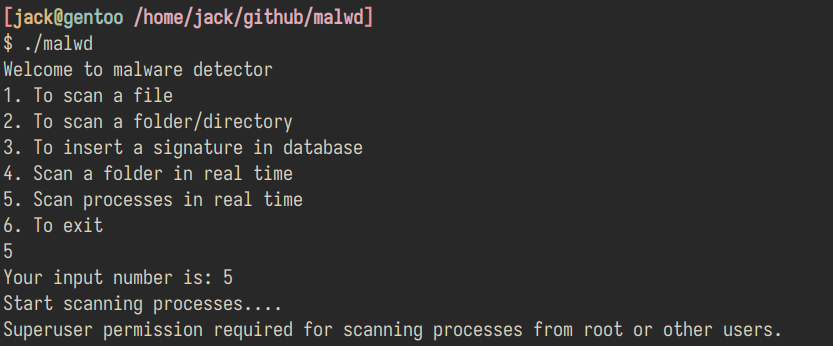
\includegraphics[width=.9\linewidth]{./images/3.png}
\caption{\label{fig:org388f7b4}Startup screen}
\end{center}
Options are self explainatory.

\begin{figure}[htbp]
\centering
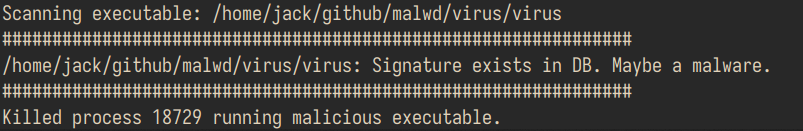
\includegraphics[width=.9\linewidth]{./images/2.png}
\caption{\label{fig:org4866208}Scanning the processes}
\end{figure}

If you choose option 5 i.e scan the running processes in real time. It will start looking at process executables in proc directory.

If it finds any suspicious executable it will try to kill that process.
\begin{figure}[htbp]
\centering
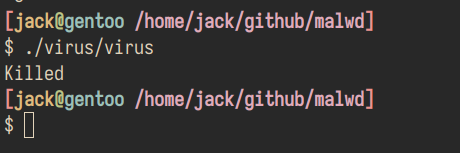
\includegraphics[width=.9\linewidth]{./images/1.png}
\caption{\label{fig:org7bacdde}Killing suspicious executable}
\end{figure}
\end{document}
